% Chương 1

\chapter{ TỔNG QUAN VỀ PID} % Tên của chương

\label{Chapter1} % Để trích dẫn chương này ở chỗ nào đó trong bài, hãy sử dụng lệnh \ref{Chapter1} 

%----------------------------------------------------------------------------------------

% Định nghĩa một số lệnh cần thiết để điều chỉnh định dạng cho một số nội dung nhất định trong bài
\newcommand{\keyword}[1]{\textbf{#1}}
\newcommand{\tabhead}[1]{\textbf{#1}}
\newcommand{\code}[1]{\texttt{#1}}
\newcommand{\file}[1]{\texttt{\bfseries#1}}
\newcommand{\option}[1]{\texttt{\itshape#1}}

%----------------------------------------------------------------------------------------

\section{Giới thiệu chung}

PID (Proportional Integral Derivative) là một cơ chế phản hồi vòng điều khiển được sử dụng rộng rãi trong các hệ thống điều khiển tự động. Bộ điều khiển PID sẽ tính toán sai số là hiệu giữa giá trị trả về của hệ thống và giá trị điểm đặt mong muốn, từ đó thực hiện giảm sai số về mức nhỏ nhất bằng cách điều chỉnh giá trị điều khiển đầu vào. Để hệ thống đạt được kết quả tốt nhất, các thông số PID sẽ được điều chỉnh theo tính chất, đặc trưng của hệ thống.
 
\section{Cơ bản về vòng điều khiển}

Xét ví dụ về một cánh tay robot có thể điều khiển chuyển động và xác định vị trí của nó. Động cơ điện được sử dụng sao cho khi cấp điện cho động cơ, cánh tay sẽ di chuyển nâng lên hoặc hạ xuống. Khi vận hành, cần điều khiển cánh tay đến một vị trí cụ thể, tuy nhiên việc cấp năng lượng đơn thuần không thể điều khiển cánh tay robot một cách chính xác bởi quán tính, trọng lực, ngoại lực tác động lên nó trong quá trình vận hành (dịch chuyển, nâng vật, hạ vật...). Chính vì thế, ta cần sử dụng một vòng điều khiển để có thể vận hành cánh tay robot với sai số nhỏ nhất có thể.

\begin{itemize}
	
	\item PV (Process Variable): Biến quá trình - vị trí của cánh tay robot.
	\item SP (Setpoint): Vị trí điều khiển mong muốn. 
	\item e (error): Sai số hệ thống, là hiệu giữa SP và PV.
	\item MV (Manipulated Variable): Biến điều khiển, là đầu ra của bộ điều khiển PID.
	
\end{itemize}

Từ việc xác định vị trí hiện tại của động cơ (PV) so với vị trí điểm đặt mong muốn, hệ thống sẽ tính toán sai số, kết hợp với các thuật toán, bộ điều khiển sẽ cung cấp cho động cơ một dòng điện phù hợp để cánh tay robot đạt được vị trí mong muốn.

\section{Cấu trúc của bộ điều khiển PID}
Tiểu luận này trình bày dạng song song của bộ điều khiển PID. Bộ điều khiển PID gồm ba thành phần: tỉ lệ, tích phân, vi phân.

\begin{figure}[h!]
	\centering
	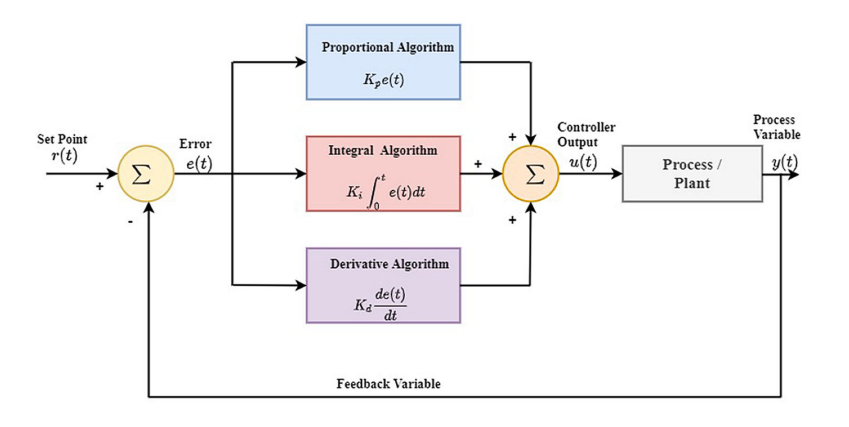
\includegraphics[width=0.8\textwidth]{cau truc pid.png}
	\caption[Cấu trúc của bộ điều khiển PID]{Cấu trúc của bộ điều khiển PID}
	\label{fig:cautrucPID}
\end{figure}

Tổng của ba thành phần này chính là đầu ra của hệ thống(MV).
\begin{align}
 	MV(t) = u(t) &= P_{out} + I_{out} + D_{out}   \\
		&= K_p.e(t) + K_i.\int_{0}^{t}e(t)dt + K_d.\frac{d}{dt}e(t)
\end{align}
    
\subsection{Thành phần tỉ lệ}

Tỷ lệ (Proportional): Làm thay đổi giá trị đầu ra tỷ lệ với giá trị sai số hiện tại. Tuy nhiên trong thực tế, do sự sai lệch nên sẽ không bao giờ đặt được đến giá trị mong muốn. Để đáp ứng tỉ lệ cần nhân sai số với độ lợi $K_p$. Độ lợi tỷ lệ cao dẫn đến sự thay đổi lớn cho đầu ra. Nếu độ lợi tỷ lệ quá cao, hệ thống có thể trở nên không ổn định. Ngược lại, độ lợi nhỏ dẫn đến phản hồi đầu ra nhỏ và bộ điều khiển kém nhạy hơn. Tỷ lệ đóng góp phần lớn sự thay đổi đầu ra.

Thành phần tỉ lệ được cho bởi:
\begin{align}
	P_{out} &= K_p.e(t)
\end{align} 
Trong đó:

\begin{itemize}
	
	\item $P_{out}$: Đầu ra của khâu tỉ lệ.
	\item $K_p$: Độ lợi tỉ lệ(là một tham số điều chỉnh).
	\item e: sai số = SP - PV.
	\item t: thời gian tức thời(hiện tại).
	
\end{itemize}

\subsection{Thành phần tích phân}

Tích phân (Integral): Khâu này tỉ lệ với biên độ sai số và thời gian xảy ra sai số. Cộng dồn các sai số tức thời theo thời gian (tích phân sai số) cho ra tích lũy sai số. Tích lũy sai số sau đó được nhân với độ lợi tích phân $K_p$. Thuật ngữ tích phân tăng tốc độ di chuyển của hệ thống về phía điểm đặt và loại bỏ lỗi trạng thái ổn định còn lại xảy ra với bộ điều khiển chỉ sử dụng thành phần tỉ lệ. Tuy nhiên, việc cộng dồn các sai số tích lũy từ quá khứ của khâu tích phân có thể khiến giá trị hiện tại vượt quá giá trị điểm đặt.

Thành phần tích phân được cho bởi:

\begin{align}
	I_{out} &= K_i.\int_{0}^{t}e(t)dt
\end{align}

Trong đó:

\begin{itemize}
	
	\item $P_{out}$: Đầu ra của khâu tích phân.
	\item $K_i$: Độ lợi tích phân(là một tham số điều chỉnh).
	\item e: sai số = SP - PV.
	\item t: thời gian tức thời(hiện tại).
	
\end{itemize}

\subsection{Thành phần đạo hàm}

Đạo hàm (Derivative): Một thành phần khác được sử dụng trong bộ điều khiển PID là đạo hàm. Tốc độ thay đổi của sai số quá trình được tính toán bằng cách xác định độ dốc của sai số theo thời gian (tức là đạo hàm bậc một theo thời gian) và nhân với độ lợi $K_p$. Đạo hàm dự đoán hành vi của hệ thống từ đó cải thiện ổn định của hệ thống.

Thành phần đạo hàm được cho bởi:

\begin{align}
	D_{out} &= K_d.\frac{d}{dt}e(t)
\end{align}

Trong đó:

\begin{itemize}
	
	\item $D_{out}$: Đầu ra của khâu tích phân.
	\item $K_d$: Độ lợi(là một tham số điều chỉnh).
	\item e: sai số = SP - PV.
	\item t: thời gian tức thời(hiện tại).
	
\end{itemize}







%----------------------------------------------------------------------------------------

\section{Một số bộ điều khiển được xây dựng từ P, I và D}

Tùy vào đặc trưng của một số hệ thống và mục đích sử dụng, có thể kết hợp các thành phần: tỷ lệ (P), tích phân (I) và đạo hàm (D) để tạo nên một số bộ điều khiển.


\subsection{Bộ điều khiển tỷ lệ tích phân}

Bộ điều khiển tỷ lệ tích phân (PI) được xây dựng bằng việc kết hợp hai thành phần tỷ lệ (P), tích phân (I) và không sử dụng thành phần đạo hàm (D) của thuật toán PID. Hệ thống PI là một hình thức kiểm soát phản hồi. Nó cung cấp thời gian phản hồi nhanh hơn so với điều khiển chỉ sử dụng thành phần tích phân (I) do bổ sung thành phần tỷ lệ (P). Điều khiển PI ngăn hệ thống dao động và điều khiển hệ thống về điểm đặt (SP).

\newpage

Đầu ra của bộ điều khiển PI:

\begin{align}
	MV(t) &= P_{out} + I_{out}    \\
	&= K_p.e(t) + K_i.\int_{0}^{t}e(t)dt 
\end{align}

\subsection{Bộ điều khiển tỷ lệ đạo hàm}

Một sự kết hợp khác của hệ thống PID là bộ điều khiển tỷ lệ đạo hàm (PD). Thành phần của bộ điều khiển gồm hai thành phần tỷ lệ (P) và đạo hàm (D), bỏ qua thành phần tích phân (I). Một hệ thống PD hoạt động trên quy trình hiện tại và dự đoán. Đầu ra điều khiển là sự kết hợp tuyến tính của tín hiệu lỗi và đạo hàm của nó.

Đầu ra của bộ điều khiển PD:

\begin{align}
	MV(t) &= P_{out} + D_{out}   \\
	&= K_p.e(t) + K_d.\frac{d}{dt}e(t)
\end{align}


\subsection{Bộ điều khiển tỷ lệ - tích phân - đạo hàm}

Như đã đề cập ở trên, bộ điều khiển PID là sự kết hợp của cả ba khâu: tỷ lệ, tích phân và đạo hàm. Hệ thống PID được sử dụng rộng rãi nhất bởi nó là sự kết hợp các ưu điểm của ba thành phần này. Mỗi thành phần có vai trò đặc trưng giúp cho hệ thống được tối ưu trong quá trình hoạt động và mang lại hiệu suất cao.

\section{Các thành phần độ lợi của hệ thống}
Với cấu trúc đơn giản và hiệu quả mang lại cao mà ngày nay điều khiển PID vẫn được sử dụng rộng rãi trong công nghiệp. Ba hằng số độ lợi: tỷ lệ ($K_p$), tích phân ($K_i$) và đạo hàm ($K_d$) có ý nghĩa quan trọng trong một hệ thống PID. Việc thay đổi các hằng số này sẽ quyết định đến đầu ra của hệ thống. Chính vì thế, một bộ điều khiển PID được "tinh chỉnh tốt" có thể mang lại hiệu suất tuyệt vời. Từ "tinh chỉnh tốt" nhấn mạnh rằng hiệu suất của bộ điều khiển PID chủ yếu phụ thuộc vào quá trình điều chỉnh \cite{aastrom2001future}. Mỗi hệ thống cần có bộ số $K_p$, $K_i$, $Kd$ khác nhau sao cho phù hợp để hệ thống hoạt động ổn định, đảm bảo hiệu suất với bài toán đặt ra.

\subsection{Độ lợi tỷ lệ}

Giá trị của độ lợi tỷ lệ ($K_p$) càng lớn thì hệ thống đáp ứng càng nhanh, tuy nhiên sai số sẽ càng lớn. Một giá trị $K_p$ quá lớn sẽ làm cho hệ thống hoạt động bị sai lệch, thiếu sự ổn định và tin cậy. Ngược lại, nếu $K_p$ quá nhỏ cũng khiến cho hệ thống hoạt động kém nhạy, dẫn đến mất tính ổn định cho toàn hệ thống.

\begin{figure}[h!]
	\centering
	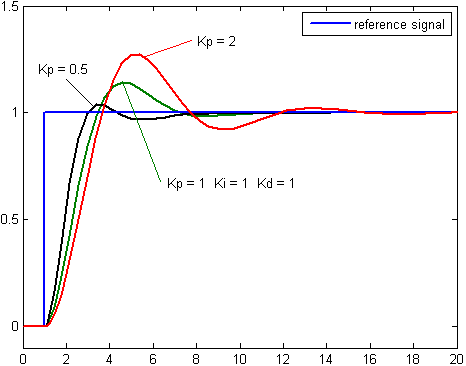
\includegraphics[width=0.8\textwidth]{Kp.png}
	\caption[Đáp ứng khâu tỷ lệ của hệ thống với $Ki$, $K_d$ không đổi]{Đáp ứng khâu tỷ lệ của hệ thống với $Ki$, $K_d$ không đổi}
	\label{fig:Đáp ứng $K_p$}
\end{figure}

\newpage

\subsection{Độ lợi tích phân}

Giá trị của độ lợi tích phân ($K_i$) càng lớn thì sai số ổn định bị triệt tiêu càng nhanh, đổi lại độ vọt lố của hệ thống càng lớn. Các giá trị sai số được tích phân trong quá trình đáp ứng của hệ thống cần phải được triệt tiêu bằng tích phân trước khi tiến tới trạng thái ổn định. 

\begin{figure}[h!]
	\centering
	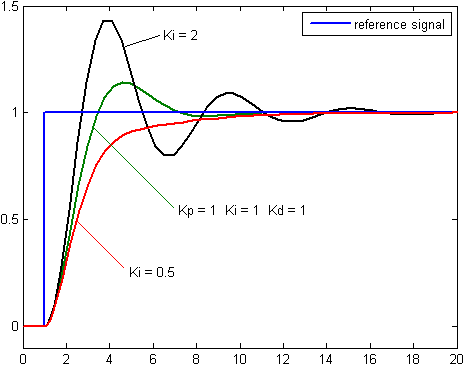
\includegraphics[width=0.8\textwidth]{Ki.png}
	\caption[Đáp ứng khâu tích phân của hệ thống với $Ki$, $K_d$ không đổi]{Đáp ứng khâu tích phân của hệ thống với $Ki$, $K_d$ không đổi}
	\label{fig:Đáp ứng $K_i$}
\end{figure}

\newpage

\subsection{Độ lợi đạo hàm}

Giá trị của độ lợi đạo hàm ($K_d$) càng lớn, độ vọt lố càng giảm nhưng lại làm chậm đáp ứng của hệ thống và có thể dẫn đến sự mất ổn định trong quá trình hoạt động của hệ thống.

\begin{figure}[h!]
	\centering
	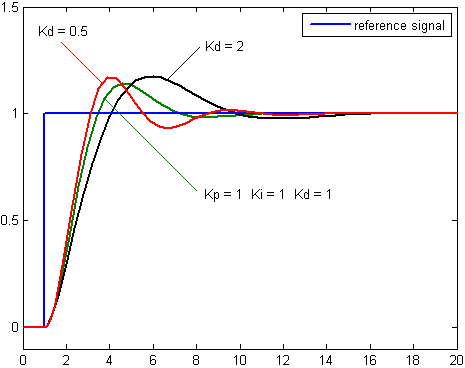
\includegraphics[width=0.8\textwidth]{Kd.png}
	\caption[Đáp ứng khâu đạo hàm của hệ thống với $Ki$, $K_d$ không đổi]{Đáp ứng khâu đạo hàm của hệ thống với $Ki$, $K_d$ không đổi}
	\label{fig:Đáp ứng $K_d$}
\end{figure}

\section{Một số phương pháp điểu chỉnh thông số PID}

Một bộ điều khiển PID phụ thuộc rất nhiều vào ba thông số độ lợi. Nếu ba thông số $K_p$, $K_i$, $K_d$ không được lựa chọn thích hợp, hệ thống sẽ hoạt động với độ tin cậy thấp, độ chính xác kém và dẫn đến sai lệch của hệ thống. Chính vì thế, cần xác định bộ số này sao cho phù hợp với hệ thống. Có nhiều phương pháp để điều chỉnh thông số PID cho một hệ thống.

\subsection{Phương pháp điều chỉnh thủ công}

Đây là phương pháp hiệu chỉnh đơn giản, dễ dàng đạt được một hệ thống có đáp ứng đầu ra như ý muốn và không cần thiết phải có mô hình chi tiết về toán học của hệ thống. Tuy nhiên phương pháp này là mất nhiều thời gian và người hiệu chỉnh cần phải có nhiều kinh nghiệm. Các bước hiệu chỉnh:

\begin{itemize}	
	\item Đầu tiên chỉnh cả ba thông số $K_p$, $K_i$, $K_d$ về 0. 
	\item Tăng dần $K_p$ cho đến khi đầu ra của vòng điều khiển dao động, sau đó $K_p$ được đặt về xấp xỉ một nửa giá trị đó.
	\item Tiếp theo, tăng giá trị $K_i$ đến giá trị phù hợp sao cho hệ thống đủ thời gian xử lý. Tuy nhiên, giá trị $K_i$ quá lớn sẽ gây mất ổn định.
	\item Cuối cùng tăng $K_d$ đến khi dao động của hệ thống bị loại bỏ. $K_d$ quá lớn sẽ khiến đáp ứng dư và vọt lố.
\end{itemize}

\subsection{Phương pháp Ziegler–Nichols 2}
Phương pháp Ziegler–Nichols được đưa ra bởi John G. Ziegler và Nathaniel B. Nichols vào những năm 1940. Các bước hiệu chỉnh bằng phương pháp này bao gồm:

\begin{itemize}
	\item Chỉnh $K_p$, $K_i$, $K_d$ về 0. 
	\item Tăng dần độ lợi $K_p$ từ 0 cho đến khi đạt được độ lợi $K_{cr}$ mà tại đó đầu ra của của vòng điều khiển dao động với biên độ không đổi.
	\begin{figure}[h!]
		\centering
		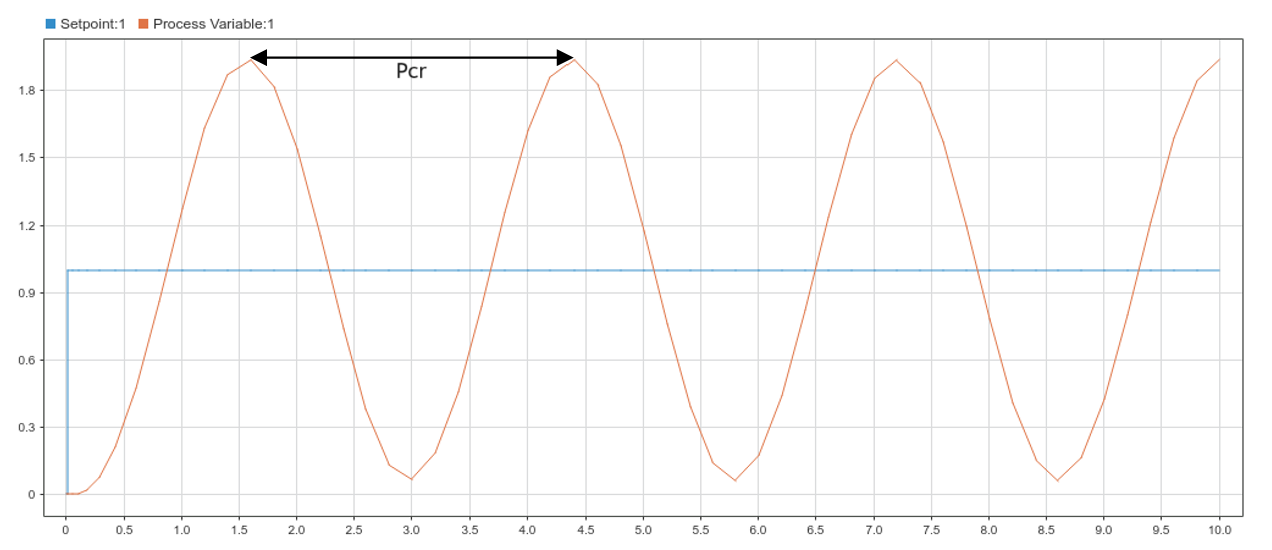
\includegraphics[width=0.8\textwidth]{Pcr.png}
		\caption[Mô tả đầu ra của hệ thống dao động với chu kỳ không đổi]{Mô tả đầu ra của hệ thống dao động với chu kỳ không đổi}
		\label{fig:Dao động của đầu ra hệ thống}
	\end{figure}
	\item Sau khi hệ dao động tuần hoàn, tiến hành xác định chu kỳ dao động $P_{cr}$ của hệ thống. Lưu ý rằng, đơn vị thời gian được lấy theo đơn vị của thời gian lấy mẫu trong hệ thống.
	
	\newpage
	
	\item Từ các giá trị $K_{cr}$ và $P_{cr}$ tìm được, có thể xác định được các giá trị $T_i$ và $T_d$ theo bảng:


	\begin{figure}[h!]
	 	\centering
		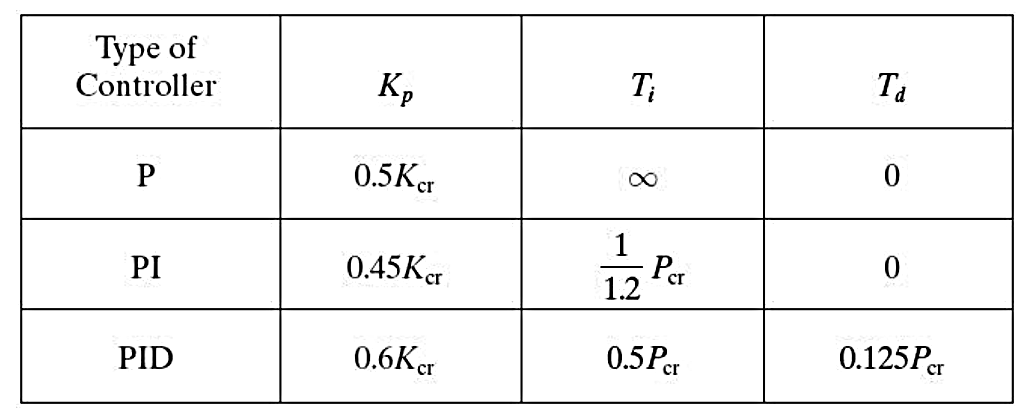
\includegraphics[width=0.8\textwidth]{Ziegler-Nichols.png}
		\caption[Bảng Ziegler-Nichols 2]{Bảng Ziegler-Nichols 2}
		\label{fig:Ziegler-Nichols 2}
	\end{figure}
	
	\item Dựa vào Ziegler-Nichols 2, các thông số $K_i$ và $K_d$ được xác định bởi:
	\begin{align}
		K_i = K_p/T_i	\\
		K_d = K_p.T_d
	\end{align}
	
	
\end{itemize}

\newpage

\subsection{Phương pháp sử dụng phần mềm chuyên dụng}

Đây là phương pháp điều chỉnh chắc chắn, chính xác. Đây là phương pháp giúp tối ưu hóa hiệu suất hệ thống, dễ dàng điều chỉnh và khả năng đáp ứng linh hoạt. Hạn chế của phương pháp này là tốn kém chi phí và cần hiểu rõ về chuyên môn cũng như hệ thống.

Dưới đây là mô tả phương pháp hiệu chỉnh độ lợi bằng cách sử dụng phần mềm Matlab Simulink. Đây là phương pháp mang lại độ tối ưu và tin cậy cao cho hệ thống. Tuy nhiên, để sử dụng phương pháp này thì cần phải đưa ra các phương trình toán học cho hệ thống, đây là một công việc đòi hỏi tính học thuật cao và khá khó khăn.

\begin{figure}[h!]
	\centering
	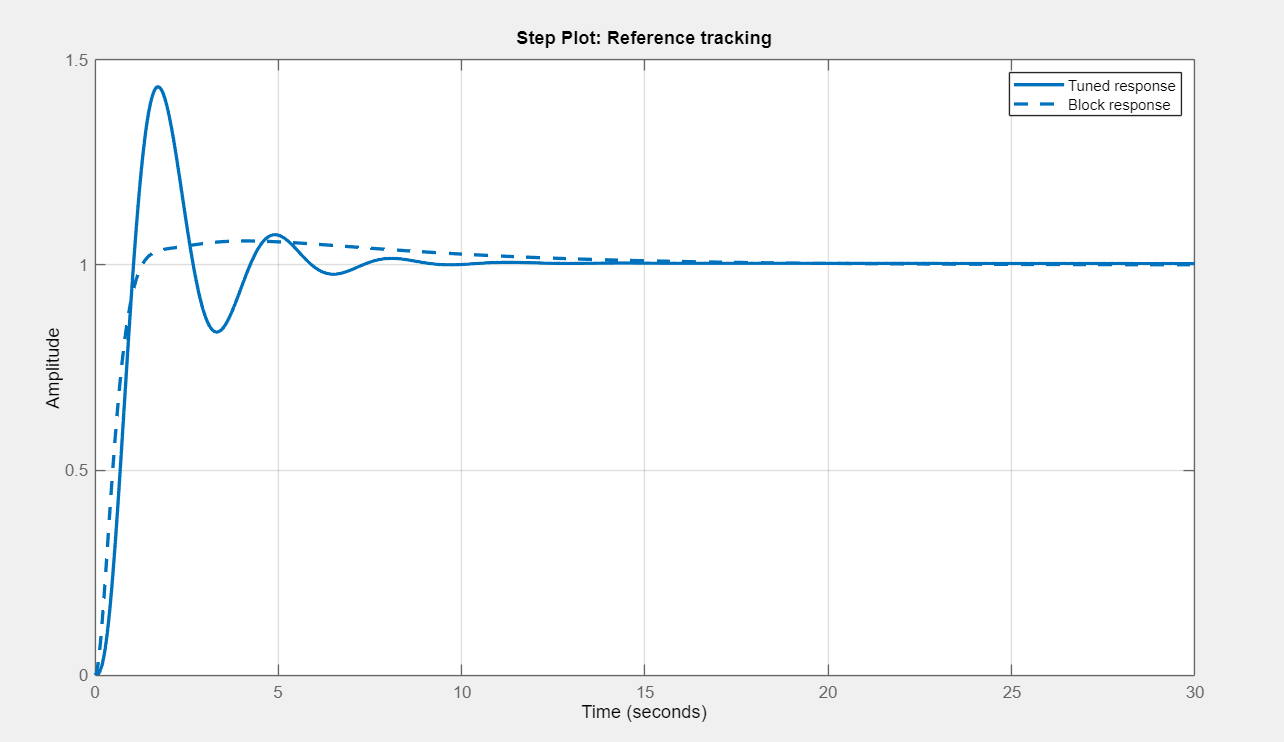
\includegraphics[width=0.8\textwidth]{tuning.png}
	\caption[Bảng hiệu chỉnh độ lợi bằng phần mềm Matlab]{Bảng hiệu chỉnh độ lợi bằng phần mềm Matlab}
	\label{fig:Hiệu chỉnh độ lợi bằng phần mềm}
\end{figure}



